This section reports the measured outcomes of the Section~\ref{sec:experiments} tests. It presents communication timing, simulation behaviour, safety outcomes, and hardware interaction observations.
Interpretation of these findings and their design implications is deferred to Section~\ref{sec:discussion}.
\subsection{Communication Performance}
Communication performance was evaluated using standalone serial tests and runtime logging of the integrated haptic application.

\subsubsection{Packet Rate and Integrity Results}
Packet rate testing showed that communication performance remained consistent over a wide range of requested transmission frequencies, although the behaviour was not uniform across all tested rates.

At lower requested rates of 100~Hz and 250~Hz, packet loss was observed, with drop fractions of approximately 20.3\% and 8.5\% respectively. In contrast, for requested rates of 500~Hz and above, no dropped packets were observed in the recorded data, as shown in Fig.~\ref{fig:comm_overview}(a), where packet loss occurs only at the lowest transmission rates. Out-of-order packets were extremely rare across all higher-rate tests, with only a single out-of-order event recorded in each case.

The measured receive rate tracked the requested transmission rate closely across the full test range. As shown in Fig.~\ref{fig:comm_overview}(b), the relationship between requested and measured rate was approximately linear, indicating that the communication system maintained throughput proportional to the commanded transmission frequency.

\begin{figure}[htbp]
	\centering
	
	\begin{subfigure}{0.48\textwidth}
		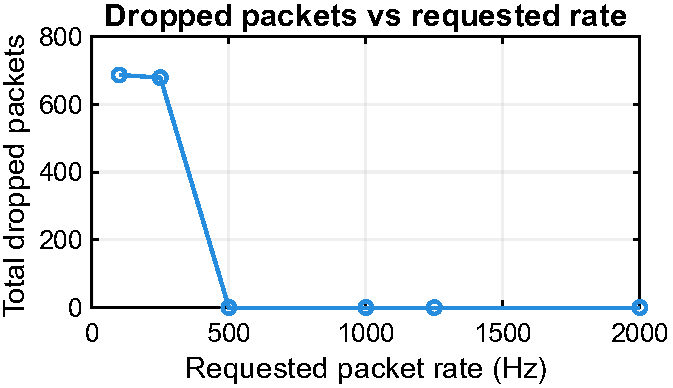
\includegraphics[width=0.95\linewidth]{images/Dropped packets vs requested rate.pdf}
		\caption{Dropped packets}
	\end{subfigure}
	\hfill
	\begin{subfigure}{0.48\textwidth}
		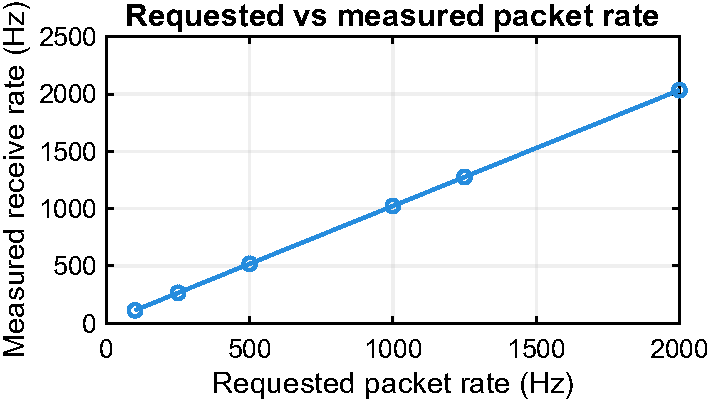
\includegraphics[width=0.95\linewidth]{images/Requested vs measured packet rate.pdf}
		\caption{Rate tracking}
	\end{subfigure}
	
	\caption{
		Communication performance across transmission rates. Packet loss occurred only at low frequencies, while measured receive rate tracked the requested rate approximately linearly.
	}
	\label{fig:comm_overview}
\end{figure}

Inter-arrival jitter, measured as the standard deviation of packet inter-arrival time, was present in all tests, with standard deviation decreasing as the requested rate increased, as shown in Fig.~\ref{fig:jitter}. However, percentile analysis revealed that occasional large timing excursions persisted even at higher rates, indicating intermittent latency spikes. While average jitter decreased with increasing rate, worst-case timing excursions remained present.

\begin{figure}[htbp]
	\centering
	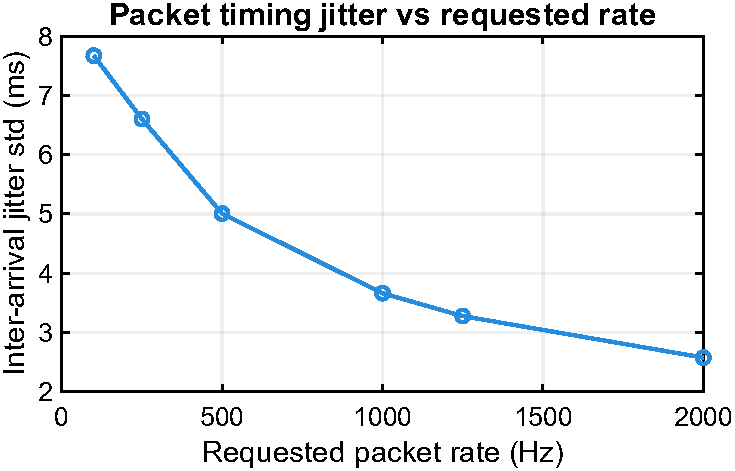
\includegraphics[width=0.58\textwidth]{images/Packet timing jitter vs requested rate.pdf}
	\caption{
		Packet inter-arrival jitter decreases with requested rate, although occasional large timing excursions remain present.
	}
	\label{fig:jitter}
\end{figure}

Overall, the serial link supported nominal packet throughput at or above 1~kHz with negligible packet loss in the tested configuration. This result describes packet generation and throughput, rather than low-latency delivery or 1\,ms closed-loop state freshness.

\subsubsection{Round-Trip Latency Results} \label{sec:results_rtt}
Round-trip latency results were highly consistent across all tested ping intervals. For nominal transmission intervals of 1~ms, 2~ms, and 10~ms, the success rate was 100\% in all cases, with no timeouts observed over 1000 samples per test.
The mean measured round-trip latency remained approximately constant across all three test conditions, with values of 15.60~ms, 15.64~ms, and 15.67~ms respectively. Similarly, the 95th and 99th percentile RTT values were tightly grouped around 16.2--16.4~ms, indicating consistent and predictable timing behaviour across repeated measurements. This behaviour is further illustrated in Fig.~\ref{fig:rtt_cdf}, where the cumulative distributions for all three tests overlap closely and rise sharply at approximately 15--16~ms, indicating that RTT is largely independent of the selected ping interval.

\begin{figure}[htbp]
	\centering
	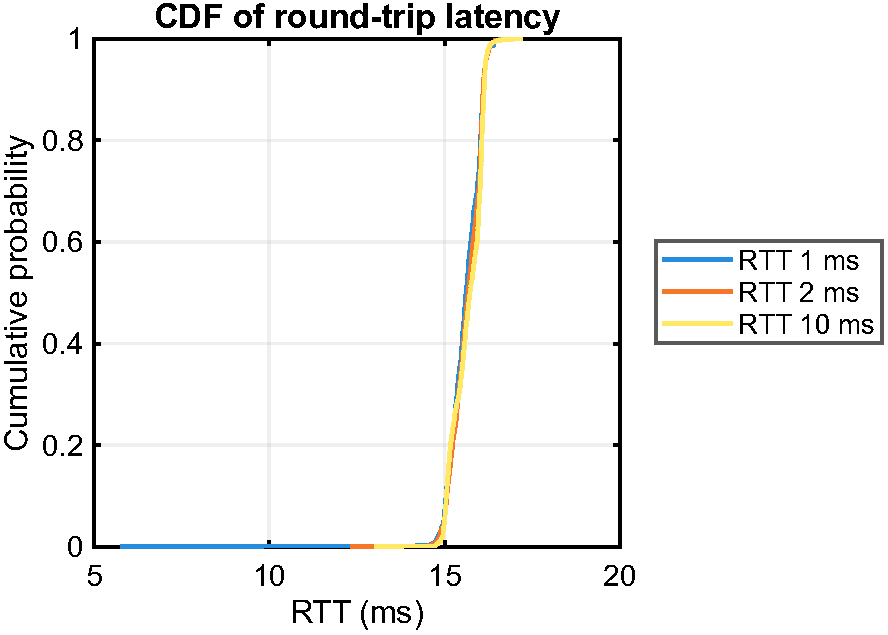
\includegraphics[width=0.6\textwidth]{images/CDF of round-trip latency.pdf}
	\caption{
		Cumulative distributions of RTT for 1~ms, 2~ms, and 10~ms ping intervals. The overlapping curves indicate a largely fixed 15--16~ms delay component.
	}
	\label{fig:rtt_cdf}
\end{figure}

The standard deviation of RTT remained below 0.52~ms in all cases, suggesting relatively low variability in round-trip timing. Minimum and maximum observed RTT values showed occasional larger deviations from the typical latency range, particularly in the 1~ms test, but these did not significantly affect the overall distribution.

These results indicate that RTT was dominated by a largely fixed delay component and changed little with ping interval. The measured delay remained predictable due to low variability and zero observed timeouts.

\subsubsection{End-to-End Host-Side Timing Results} \label{sec:results_host_timing}
End-to-end timing behaviour of the integrated haptic pipeline was evaluated using runtime logging of matched state-command cycles and raw parsed state packets.

Analysis of \texttt{device\_timing.csv} showed that all recorded control cycles were successfully matched, with a matched fraction of 1.000, indicating consistent correspondence between received state packets and transmitted torque commands.

The host-side end-to-end latency, defined as the time between state-packet parsing and completion of torque command transmission, was found to be low. The mean latency was 0.299~ms, with a median of 0.104~ms. The 95th percentile latency was 0.546~ms, and the 99th percentile was 2.04~ms, with a maximum observed latency of 3.35~ms. As shown in Fig.~\ref{fig:e2e_hist}, the distribution was concentrated at low values, with prominent peaks near 0~ms and around 0.5~ms, and only a limited number of higher-latency events.

\begin{figure}[htbp]
	\centering
	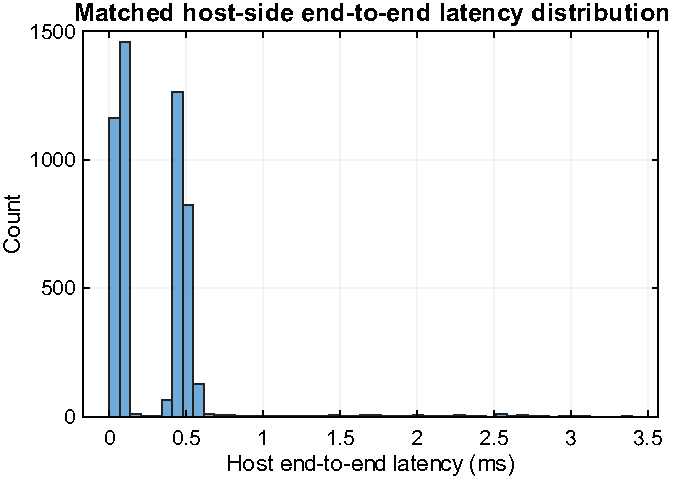
\includegraphics[width=0.64\textwidth]{images/Matched host-side end-to-end latency distribution.pdf}
	\caption{
		Matched host-side latency from state-packet parsing to torque-command transmission, concentrated at low values with few higher-latency outliers.
	}
	\label{fig:e2e_hist}
\end{figure}

Breakdown of intermediate pipeline delays showed that the majority of this latency was associated with serial transmission. The mean transmission duration was 0.249~ms, while the delay associated with publishing tool state and processing the haptic pipeline remained small, with mean values of 0.024~ms and 0.0044~ms respectively. This indicates that host-side computation and message-passing overhead were negligible relative to communication time.

Sequence analysis showed that command sequence progression remained consistent, with a mean command sequence gap of 1.14 and a maximum of 6, indicating that command updates were generally applied sequentially with minimal skipping. In contrast, the matched state sequence gap was significantly larger, with a mean of 33.45. This reflects the fact that the control loop operated on a subset of the available incoming state packets rather than processing every parsed packet. Here, sequence gap denotes the difference between consecutive sequence identifiers, such that a value of 1 corresponds to consecutive packets or commands and larger values indicate skipped intermediate sequence numbers.

A total of 54\,161 valid state packets were parsed during the test, compared to 5\,048 matched control cycles, confirming that the control loop operated on a subset of the incoming packet stream rather than consuming every parsed packet. The estimated parsed packet rate, computed from the mean host-side inter-arrival time, was approximately 1006~Hz, which is close to the expected 1~kHz transmission rate.

Analysis of host-side parsed-packet inter-arrival timing revealed significant variability. The mean inter-arrival time was 0.994~ms, but the median was only 0.0016~ms, reflecting that many packets were processed in immediate succession within bursts. The large difference between mean and median inter-arrival time indicates that packets were frequently processed in rapid bursts following periods of delay, rather than arriving at uniform intervals. This behaviour is illustrated in Fig.~\ref{fig:raw_host_hist}, where a dominant peak near 0~ms is accompanied by a much smaller secondary concentration around 14--16~ms. The 95th and 99th percentile inter-arrival times were 14.5~ms and 15.8~ms respectively, confirming the presence of intermittent host-side stalls.

\begin{figure}[htbp]
	\centering
	\includegraphics[width=1.0\textwidth]{images/Raw parsed state packet inter-arrival distribution(final).pdf}
	\caption{
		Host-side parsed-packet inter-arrival distribution. The secondary peak corresponds to the 95th--99th percentile range of 14.5--15.8~ms.
	}
	\label{fig:raw_host_hist}
\end{figure}

Despite this non-uniform host-side processing pattern, analysis of MCU-side timestamps showed that the embedded system generated state packets at a consistent rate. The effective MCU period per state was approximately 1.00~ms, corresponding to a nominal packet generation rate of 1000~Hz, with very low variability.

Taken together, the embedded controller generated packets at a regular rate, while host-side packet timing was non-uniform. Host-side processing latency nevertheless remained low. These results separate local packet generation and host computation from the effective age of the state used for haptic feedback.

\subsection{Simulation Validation Results}

Simulation validation was performed as described in Section~\ref{sec:method_simulation}, with actuator output disabled. These tests evaluated the haptic rendering model independently of physical actuator dynamics.

\subsubsection{Virtual Wall Contact Response} \label{sec:results_virtual_wall}

The virtual wall response was evaluated using a single-depth hold test. During contact, the rendered force magnitude had a mean value of 11.46~N and a standard deviation of 0.30~N, corresponding to a coefficient of variation of 0.026.

As shown in Fig.~\ref{fig:single_depth_contact}, force was generated only when the end-effector penetrated the virtual wall. When the end-effector was outside the wall, the output force remained approximately zero.

\begin{figure}[htbp]
	\centering
	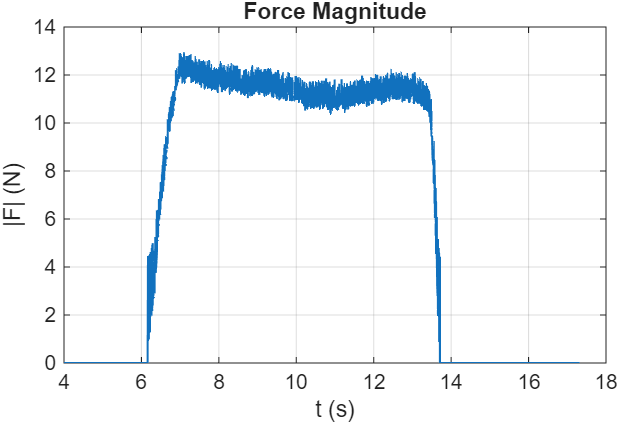
\includegraphics[width=0.58\textwidth]{images/SingleDepth_Force_Vs_Time.png}
	\caption{
		Single-depth virtual wall contact test. The rendered \( |\mathbf{F}| \) remains steady during sustained contact, with mean 11.46~N, standard deviation 0.30~N, and coefficient of variation 0.026.
	}
	\label{fig:single_depth_contact}
\end{figure}

\subsubsection{Force--Penetration Characterisation} \label{sec:results_force_penetration}

A multi-depth hold test was used to quantify the relationship between virtual penetration depth and logged rendered-force magnitude. A linear fit to the force--penetration data produced an effective stiffness of 489.57~N\,m$^{-1}$ with $R^2 = 0.9973$, as shown in Fig.~\ref{fig:force_penetration_fit}.

This closely matches the configured virtual coupling stiffness of 500~N\,m$^{-1}$ over the tested range.

\begin{figure}[htbp]
	\centering
	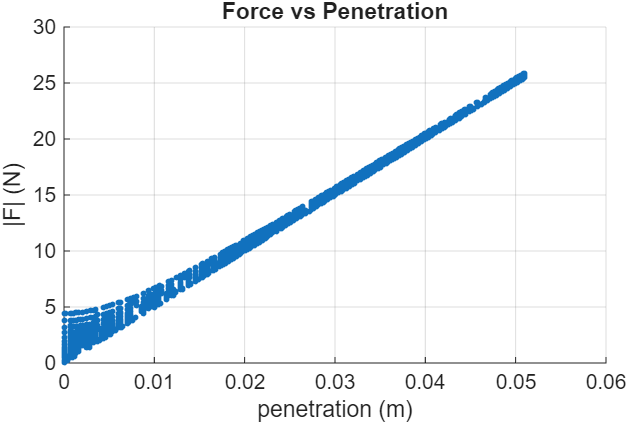
\includegraphics[width=0.58\textwidth]{images/MultiDepth_Force_Vs_Pen.png}
	\caption{
		Force--penetration relationship from the multi-depth hold test, with fitted stiffness 489.57~N\,m$^{-1}$ and $R^2 = 0.9973$.
	}
	\label{fig:force_penetration_fit}
\end{figure}

\subsubsection{Free-Space and Saturation Behaviour}

A no-contact test verified that the haptic engine produced no significant force output in free space.

A deep-penetration test was also performed to verify host-side force limiting. Under large penetration, the commanded force saturated at approximately 31~N, as shown in Fig.~\ref{fig:force_saturation}.

\begin{figure}[htbp]
	\centering
	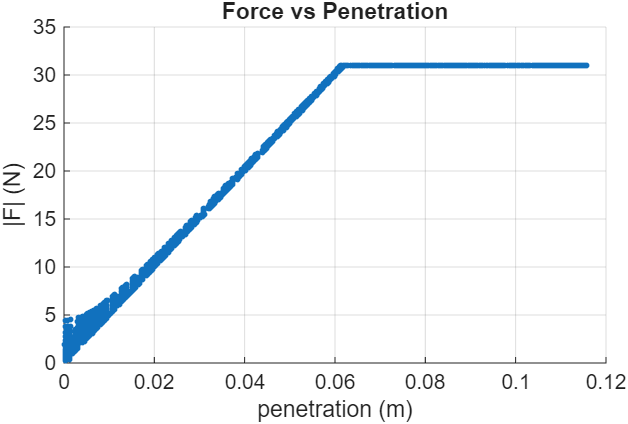
\includegraphics[width=0.58\textwidth]{images/Saturated_Force_Vs_Pen.png}
	\caption{
		Deep-penetration simulation test showing force saturation at the host-side limit of approximately 31~N.
	}
	\label{fig:force_saturation}
\end{figure}


\subsection{Safety Validation Results}

Safety validation evaluated whether torque commands remained bounded during high-force contact, rapid command transitions, and communication loss.

\subsubsection{Torque Saturation}

Torque saturation was evaluated using the deep-penetration test. Host-side saturation occurred in 31.10\% of samples, with the maximum raw torque command reaching 9.35~N\,m before being clamped to 7.66~N\,m. On the device side, the maximum applied torque was limited to 6.50~N\,m, matching the configured firmware torque cap.

\begin{figure}[htbp]
	\centering
	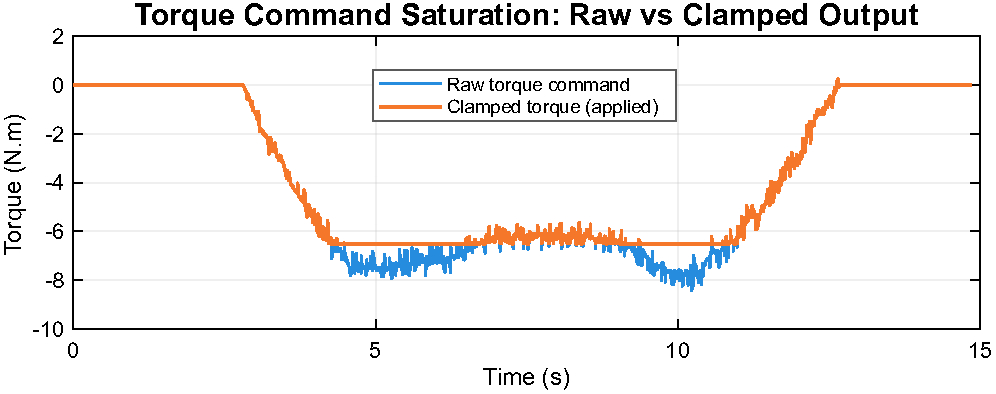
\includegraphics[width=0.65\textwidth]{images/Command and Applied Torque.pdf}
	\caption{
		Torque saturation during deep-penetration testing: raw host commands are clamped before transmission and applied torque remains bounded by the 6.50~N\,m firmware cap.
	}
	\label{fig:torque_saturation}
\end{figure}

\subsubsection{Rate Limiting} \label{sec:results_rate_limiting}

The embedded torque slew-rate limiter was evaluated from the applied torque logs. The measured 95th percentile slew rate was 55.000~N\,m\,s$^{-1}$, the 99th percentile was 55.005~N\,m\,s$^{-1}$, and the maximum measured slew rate was 55.010~N\,m\,s$^{-1}$. These values closely match the configured firmware limit of 55~N\,m\,s$^{-1}$.

The slew-rate distribution is shown in Fig.~\ref{fig:slew_hist}. The dominant peak at 0~N\,m\,s$^{-1}$ corresponds to steady-state operation, while the sharp upper bound occurs at the configured 55~N\,m\,s$^{-1}$ limit.

\begin{figure}[htbp]
	\centering
	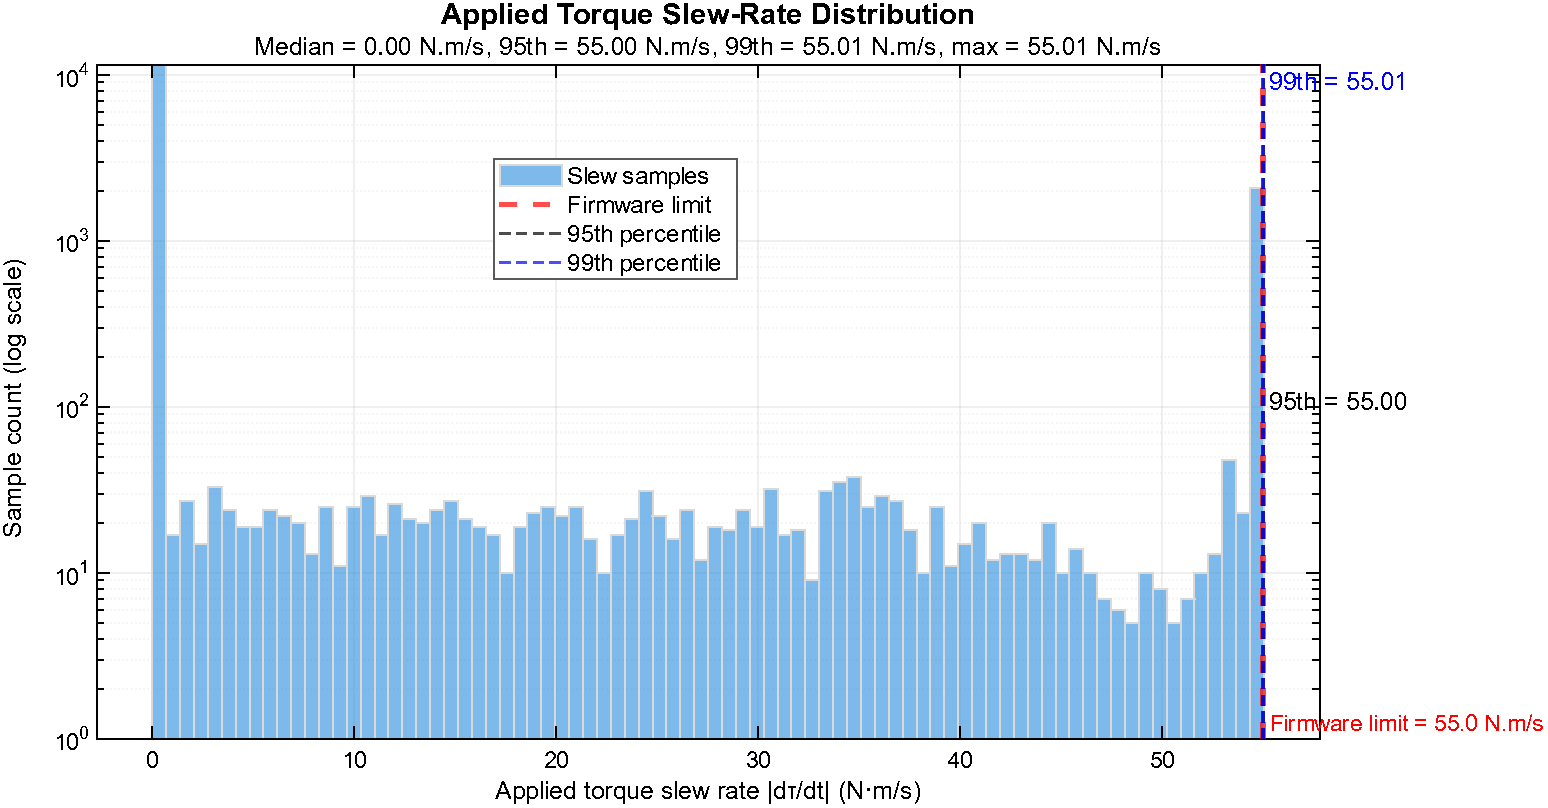
\includegraphics[width=0.74\textwidth]{images/Torque Slew Rate Distribution.pdf}
	\caption{
		Applied torque slew-rate histogram showing a sharp upper bound at the firmware limit of 55~N\,m\,s$^{-1}$.
	}
	\label{fig:slew_hist}
\end{figure}

\subsubsection{Watchdog Timeout Behaviour}

The watchdog was evaluated by deliberately interrupting host torque-command transmission. A total of 259 watchdog activation events were recorded, corresponding to 6.81\% of device samples. The total watchdog-active time was 0.529~s, with a mean activation duration of 0.0020~s and a maximum duration of 0.311~s.

As shown in Fig.~\ref{fig:watchdog}, applied torque was removed during watchdog activation.

\begin{figure}[htbp]
	\centering
	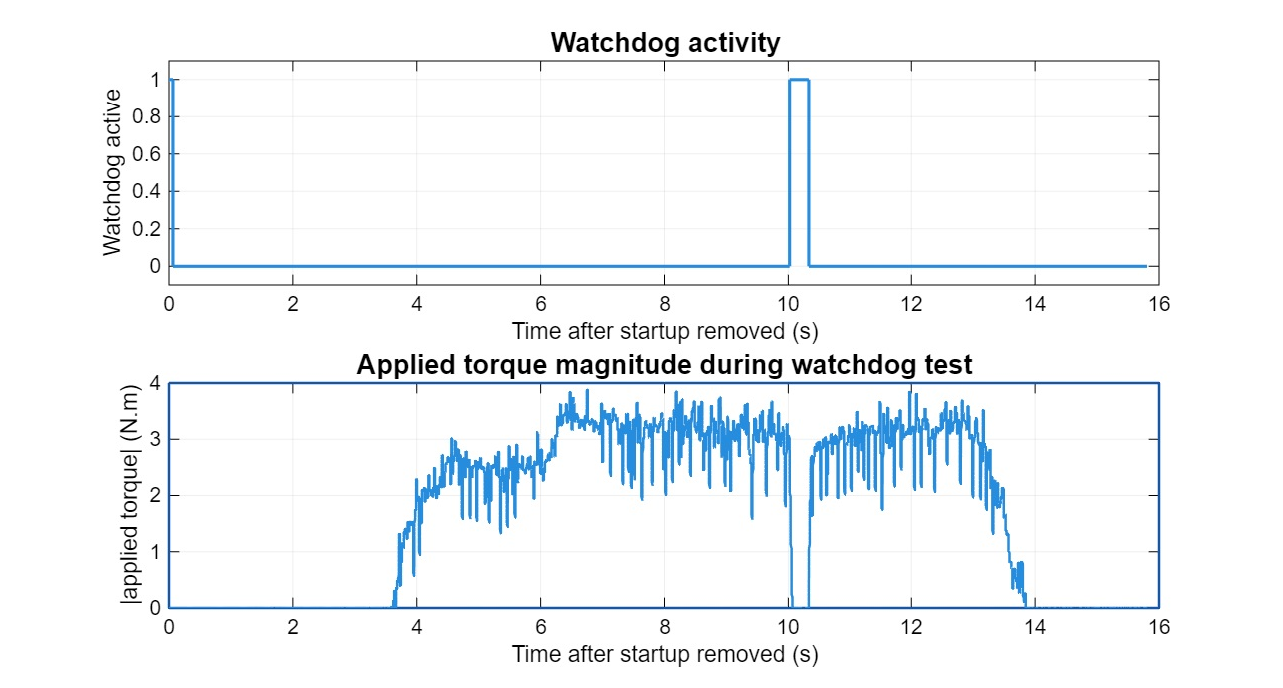
\includegraphics[width=0.74\textwidth]{images/Device Safety Validation - Watchdog Focus.pdf}
	\caption{
		Watchdog validation during interrupted host command transmission. Applied torque is removed when the watchdog becomes active.
	}
	\label{fig:watchdog}
\end{figure}

\subsubsection{Command Consistency}

Sequence-matched host and device logs showed a mean applied torque magnitude error of 0.134~N\,m between host commands and device-side applied torque. For typical commanded torques of approximately 2--4~N\,m, this corresponds to roughly 3--7\% error. Larger differences occurred during transient command changes, especially when the slew-rate limiter and safety clamps were active.


\subsection{Hardware Validation Results}

Hardware validation was performed with actuator feedback enabled. Because direct force sensing and current measurement were not available, these results quantify interaction behaviour using logged position, force-command, and torque-command data rather than calibrated physical force output. Final force-feedback testing was limited to single-axis actuation due to actuator failure, although both joints remained available for position sensing.

\subsubsection{Repeated Contact With Virtual Wall} \label{sec:results_stable_contact_hardware}

During repeated motor-enabled contact with the virtual wall, penetration remained bounded. The mean penetration depth was 0.0342~m, the 95th percentile penetration depth was 0.0498~m, and the maximum penetration depth was 0.0517~m.

The force--penetration relationship during this test remained approximately linear, with an effective stiffness of 490.99~N\,m$^{-1}$ and $R^2 = 0.9979$. This indicates that the rendered force command remained consistent with the virtual coupling model during closed-loop interaction.
The fitted stiffness of 490.99~N\,m$^{-1}$ agrees closely with the simulation-only result of 489.57~N\,m$^{-1}$ in Section~\ref{sec:results_force_penetration}. This comparison is based on logged command data rather than direct force measurement.

\begin{figure}[htbp]
	\centering
	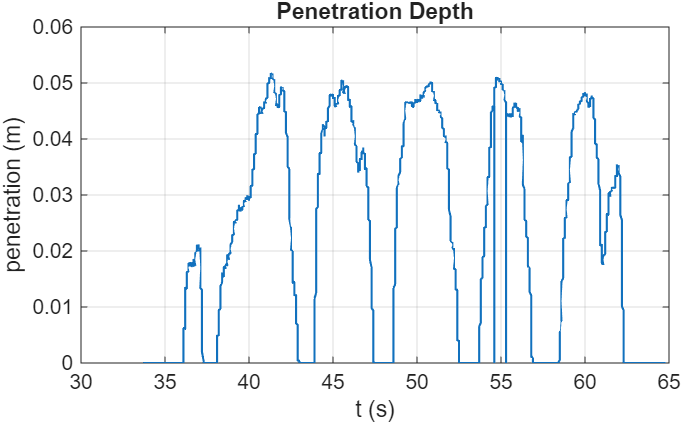
\includegraphics[width=0.58\textwidth]{images/MotorON_Pen_vs_Tine.png}
	\caption{
		Motor-enabled repeated contact test. Maximum penetration was approximately 0.052~m; the force--penetration fit gave 490.99~N\,m$^{-1}$ with $R^2=0.9979$.
	}
	\label{fig:motor_contact_penetration}
\end{figure}

\subsubsection{Constrained Motion Along a Surface}

Constrained motion was evaluated by bringing the end-effector into contact with the virtual wall and moving along the surface. Metrics were computed over the sustained-contact window from 20.50~s to 23.20~s, excluding entry and release transients. During this window, the mean penetration depth, computed from device--proxy separation, was 0.0492~m and the maximum penetration depth was 0.0512~m.

Force decomposition showed that the rendered force was predominantly normal to the surface, with a median $|F_n|/|F_t|$ ratio of 17.72 and a 95th percentile ratio of 266.03. The sustained-contact force magnitude had a mean value of 24.68~N and a standard deviation of 0.72~N, corresponding to a coefficient of variation of 0.029.

The device and proxy trajectories are shown in Fig.~\ref{fig:constrained_motion_traj}. The proxy remains aligned with the virtual wall, while the device trajectory shows bounded displacement normal to the wall and motion along the tangential direction.

\begin{figure}[H]
	\centering
	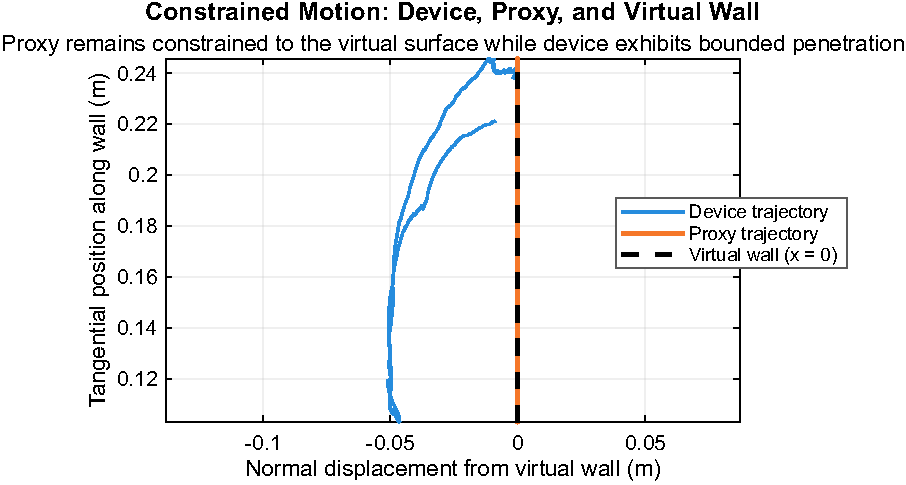
\includegraphics[width=0.7\textwidth]{images/Constrained Motion - Device, Proxy, and Virtual Wall.pdf}
	\caption{
		Device and proxy trajectories during the analysed constrained-motion window from 20.50~s to 23.20~s. The proxy remains constrained to the wall while device normal displacement stays bounded.
	}
	\label{fig:constrained_motion_traj}
\end{figure}

Across the motor-enabled hardware tests, penetration remained bounded and logged force-command behaviour remained approximately consistent with the implemented virtual coupling model.
